
\exo

\begin{enumerate}
\item On considère une fonction $f$ dont la courbe représentative est donnée ci-dessous :
\begin{center}
\def\xmin{-3}
\def\xmax{7}
\def\ymin{-2}
\def\ymax{4}
\def\xunite{0.75cm}
\def\yunite{0.75cm}
\psset{unit=\xunite, xunit=\xunite, yunit=\yunite, algebraic=true, dimen=middle, dotstyle=*, dotsize=3pt 0, linewidth=0.8pt, arrowsize=3pt 2, arrowinset=0.25, comma=true}
\begin{pspicture*}(\xmin,\ymin)(\xmax,\ymax)
\psgrid[xunit=\xunite, yunit=\yunite, subgriddiv=0, gridlabels=0, gridcolor=lightgray](0,0)(\xmin,\ymin)(\xmax,\ymax)
\psaxes[labels=none,labelFontSize=\scriptstyle, xAxis=true, yAxis=true, Dx=1, Dy=1, ticksize=-2pt 0, subticks=1]{->}(0,0)(\xmin,\ymin)(\xmax,\ymax)[{\footnotesize $x$},135][{\footnotesize $y$},-45]
\psplot[linewidth=1.2pt, plotpoints=200]{-2}{6}{3-0.25*(x-2)*(x-2)}
\begin{footnotesize}
\rput(5.5,1.5){$\cC_f$}
\uput{5pt}[225](0,0){$0$}
\uput{4pt}[270](1,0){$1$}
\uput{4pt}[180](0,1){$1$}
\end{footnotesize}
\end{pspicture*}
\end{center}
Décrire par des phrases les variations de $f$, puis dresser son tableau de variation.
\item Reprendre ces questions avec les fonctions $g$ et $h$ représentées ci-dessous :
\begin{center}
\def\xmin{-5}
\def\xmax{5}
\def\ymin{-3}
\def\ymax{3}
\def\xunite{0.75cm}
\def\yunite{0.75cm}
\psset{unit=\xunite, xunit=\xunite, yunit=\yunite, algebraic=true, dimen=middle, dotstyle=*, dotsize=3pt 0, linewidth=0.8pt, arrowsize=3pt 2, arrowinset=0.25, comma=true}
\begin{pspicture*}(\xmin,\ymin)(\xmax,\ymax)
\psgrid[xunit=\xunite, yunit=\yunite, subgriddiv=0, gridlabels=0, gridcolor=lightgray](0,0)(\xmin,\ymin)(\xmax,\ymax)
\psaxes[labels=none,labelFontSize=\scriptstyle, xAxis=true, yAxis=true, Dx=1, Dy=1, ticksize=-2pt 0, subticks=1]{->}(0,0)(\xmin,\ymin)(\xmax,\ymax)[{\footnotesize $x$},135][{\footnotesize $y$},-45]
\psplot[linewidth=1.2pt, plotpoints=200]{-4}{4}{x*x*x/6-2*x}
\begin{footnotesize}
\rput(4,-1.5){$\cC_g$}
\uput{5pt}[225](0,0){$0$}
\uput{4pt}[270](1,0){$1$}
\uput{4pt}[180](0,1){$1$}
\end{footnotesize}
\end{pspicture*}
~
\def\xmin{-1}
\def\xmax{9}
\def\ymin{-3}
\def\ymax{3}
\def\xunite{0.75cm}
\def\yunite{0.75cm}
\psset{unit=\xunite, xunit=\xunite, yunit=\yunite, algebraic=true, dimen=middle, dotstyle=*, dotsize=3pt 0, linewidth=0.8pt, arrowsize=3pt 2, arrowinset=0.25, comma=true}
\begin{pspicture*}(\xmin,\ymin)(\xmax,\ymax)
\psgrid[xunit=\xunite, yunit=\yunite, subgriddiv=0, gridlabels=0, gridcolor=lightgray](0,0)(\xmin,\ymin)(\xmax,\ymax)
\psaxes[labels=none,labelFontSize=\scriptstyle, xAxis=true, yAxis=true, Dx=1, Dy=1, ticksize=-2pt 0, subticks=1]{->}(0,0)(\xmin,\ymin)(\xmax,\ymax)[{\footnotesize $x$},135][{\footnotesize $y$},-45]
\psplot[linewidth=1.2pt, plotpoints=200]{0}{8}{2*cos(1.58*x)}
\begin{footnotesize}
\rput(7,2){$\cC_h$}
\uput{5pt}[225](0,0){$0$}
\uput{4pt}[270](1,0){$1$}
\uput{4pt}[180](0,1){$1$}
\end{footnotesize}
\end{pspicture*}
\end{center}
\end{enumerate}

\exo

\begin{enumerate}
\item On considère une fonction $f$ dont le tableau de variation est donné ci-dessous :
\begin{center}
\begin{tikzpicture}
\tkzTabInit[lgt=2,espcl=3]{$x$/0.8,$f(x)$/1.4}{$-5$, $0$, $1$, $2$}
\tkzTabVar{-/$2$,+/$5$,-/$-4$,+/$-1$}
\end{tikzpicture}
\end{center}
\begin{enumerate}
\item Donner l'ensemble de définition de $f$.
\item Décrire par des phrases les variations de $f$.
\item Tracer une courbe pouvant représenter la fonction $f$.
\end{enumerate}
\item Reprendre ces questions avec la fonction $g$ dont le tableau de variation est le suivant :
\begin{center}
\begin{tikzpicture}
\tkzTabInit[lgt=2,espcl=3]{$x$/0.8,$g(x)$/1.4}{$-4$, $-1$, $2$, $5$}
\tkzTabVar{+/$2$,-/$-3$,+/$3$,-/$-1$}
\end{tikzpicture}
\end{center}
\end{enumerate}

\exo

Soit $f$ une fonction définie sur l'intervalle $\intff{-2}{7}$. On sait que :
\begin{itemize}
\item $f$ est  croissante sur $\intff{-2}{5}$ et sur $\intff{6}{7}$, et  décroissante sur $\intff{5}{6}$ ;
\item $f(-2)=f(6)=-1$ et $f(5)=f(7)=1$.
\end{itemize}
Construire le tableau de variation de $f$, puis tracer dans un repère une courbe pouvant représenter $f$.

\exo

Indiquer si chaque affirmation est vraie ou fausse, en justifiant la réponse choisie.

Soit $f$ une fonction définie sur $\R$.

\begin{enumerate}
\item Si la fonction $f$ n'est pas  croissante sur $\R$, alors elle est  décroissante sur $\R$.
\item Si la fonction $f$ est  croissante sur $\intff{-5}{5}$, alors elle est  croissante sur $\intff{-1}{1}$.
\item Si la fonction $f$ est  croissante sur $\intff{-5}{0}$ et  décroissante sur $\intff{0}{5}$, alors $f(-5)=f(5)$.
\end{enumerate}

\exo

Soit $f$ une fonction définie sur l'intervalle $\intff{-5}{5}$.

Sur la figure ci-dessous, la courbe représentative de $f$ est tracée sur l'intervalle $\intff{0}{5}$ :
\begin{center}
\def\xmin{-6}
\def\xmax{6}
\def\ymin{-4}
\def\ymax{4}
\def\xunite{0.6cm}
\def\yunite{0.6cm}
\psset{unit=\xunite, xunit=\xunite, yunit=\yunite, algebraic=true, dimen=middle, dotstyle=*, dotsize=3pt 0, linewidth=0.8pt, arrowsize=3pt 2, arrowinset=0.25, comma=true}
\begin{pspicture*}(\xmin,\ymin)(\xmax,\ymax)
\psgrid[xunit=\xunite, yunit=\yunite, subgriddiv=0, gridlabels=0, gridcolor=lightgray](0,0)(\xmin,\ymin)(\xmax,\ymax)
\psaxes[labels=none,labelFontSize=\scriptstyle, xAxis=true, yAxis=true, Dx=1, Dy=1, ticksize=-2pt 0, subticks=1]{->}(0,0)(\xmin,\ymin)(\xmax,\ymax)[{\footnotesize $x$},135][{\footnotesize $y$},-45]
\psplot[linewidth=1.2pt, plotpoints=200]{0}{5}{x*x*x*2/9-x*x}
\begin{footnotesize}
\rput(5,-3){$\cC_f$}
\uput{5pt}[225](0,0){$0$}
\uput{4pt}[270](1,0){$1$}
\uput{4pt}[180](0,1){$1$}
\end{footnotesize}
\end{pspicture*}
\end{center}
\begin{enumerate}
\item Dans cette question, on suppose que la courbe $\cC_f$ est symétrique par rapport à l'axe des ordonnées.
\begin{enumerate}
\item Compléter en couleur le tracé de la courbe $\cC_f$.
\item Dresser le tableau de variation de $f$.
\end{enumerate}

\item Reprendre la question \textbf{1} en supposant cette fois que la courbe $\cC_f$ est symétrique par rapport à l'origine du repère (compléter le tracé en utilisant une autre couleur).
\end{enumerate}

\exo

\vspace{-12pt}
\setlength{\columnsep}{1cm}
\setlength{\columnseprule}{0pt}
\begin{multicols}{2}
On désigne par $x$ un réel compris entre $0$ et $10$, et on considère la figure ci-contre.
\begin{enumerate}
\item Lorsque $x$ augmente de $0$ à $10$, que peut-on conjecturer pour l'aire du demi-disque coloré en gris clair ? Et pour l'aire du demi-disque coloré en gris foncé ?
\end{enumerate}
\begin{center}
\def\xmin{-1}
\def\xmax{11}
\def\ymin{-1.7}
\def\ymax{5.1}
\def\xunite{0.5cm}
\def\yunite{0.5cm}
\psset{unit=\xunite, xunit=\xunite, yunit=\yunite, algebraic=true, dimen=middle, dotstyle=*, dotsize=3pt 0, linewidth=0.8pt, arrowsize=3pt 2, arrowinset=0.25, comma=true}
\begin{pspicture*}(\xmin,\ymin)(\xmax,\ymax)
%\psgrid[xunit=\xunite, yunit=\yunite, subgriddiv=0, gridlabels=0, gridcolor=lightgray](0,0)(\xmin,\ymin)(\xmax,\ymax)
%\psaxes[labelFontSize=\scriptstyle, xAxis=true, yAxis=true, Dx=1, Dy=1, ticksize=-2pt 0, subticks=1]{->}(0,0)(\xmin,\ymin)(\xmax,\ymax)[{\footnotesize $x$},135][{\footnotesize $y$},-45]
\psarc(5,0){5}{0}{180}
\pswedge[fillstyle=solid, fillcolor=lightgray!50](1.5,0){1.5}{0}{180}
\pswedge[fillstyle=solid, fillcolor=gray](6.5,0){3.5}{0}{180}
\psline{<->}(0,-0.3)(3,-0.3)
\psline{<->}(0,-1)(10,-1)
\begin{footnotesize}
\uput{3pt}[270](1.5,-0.3){$x$}
\uput{3pt}[270](5,-1){$10$}
\end{footnotesize}
\end{pspicture*}
\end{center}
\end{multicols}
\begin{enumerate}[start=2]
\item On note $f$, $g$ et $h$ les fonctions définies sur $\intff{0}{10}$ et qui, à tout $x$ de l'intervalle $\intff{0}{10}$, associent respectivement l'aire du demi-disque coloré en gris clair, l'aire du demi-disque coloré en gris foncé, et l'aire du domaine coloré.

Ces trois fonctions sont représentées ci-dessous :
\begin{center}
\def\xmin{-1.5}
\def\xmax{11.5}
\def\ymin{-10}
\def\ymax{50}
\def\xunite{0.5cm}
\def\yunite{0.075cm}
\psset{unit=\xunite, xunit=\xunite, yunit=\yunite, algebraic=true, dimen=middle, dotstyle=*, dotsize=3pt 0, linewidth=0.8pt, arrowsize=3pt 2, arrowinset=0.25, comma=true}
\begin{pspicture*}(\xmin,\ymin)(\xmax,\ymax)
%\psgrid[xunit=\xunite, yunit=\yunite, subgriddiv=0, gridlabels=0, gridcolor=lightgray](0,0)(\xmin,\ymin)(\xmax,\ymax)
\psaxes[labelFontSize=\scriptstyle, xAxis=true, yAxis=true, Dx=1, Dy=10, ticksize=-2pt 0, subticks=1]{->}(0,0)(0,0)(11,\ymax)
\psplot[linewidth=1.2pt, plotpoints=200]{0}{10}{PI*(x/2)^2/2}
\psplot[linewidth=1.2pt, plotpoints=200]{0}{10}{PI*((10-x)/2)^2/2}
\psplot[linewidth=1.2pt, plotpoints=200]{0}{10}{PI*(x/2)^2/2+PI*((10-x)/2)^2/2}
\begin{footnotesize}
\rput(5,25){$\cC_1$}
\rput(2,5){$\cC_2$}
\rput(8,5){$\cC_3$}
\end{footnotesize}
\end{pspicture*}
\end{center}
\begin{enumerate}
\item Associer à chaque fonction $f$ et $g$ sa courbe représentative.
\item En déduire la courbe qui représente la fonction $h$.
\item Avec la précision permise par le graphique, décrire les variations de la fonction $h$.
\end{enumerate}
\end{enumerate}

\exo

Soit $f$ une fonction définie sur l'intervalle $\intff{0}{6}$. Bob affirme :
\begin{center}
\og Si $f(0)> f(6)$, alors $f$ est  décroissante sur l'intervalle $\intff{0}{6}$. \fg{} 
\end{center}
\begin{enumerate}
\item Cette affirmation est-elle vraie ou fausse ?
\item La réciproque de cette affirmation est-elle vraie ou fausse ?
\end{enumerate}

\exo

On considère la fonction $g$ définie sur l'intervalle $\intff{-1}{8}$ par $g(x)=-2x^2+20x+19$.
\begin{enumerate}
\item À l'aide de la calculatrice, construire le tableau de valeurs de $g$, pour $x$ variant de $-1$ à $8$ avec un pas égal à $1$.
\item Afficher la courbe représentative de $g$ à l'écran (choisir une fenêtre d'affichage permettant de visualiser toute la courbe).
\item 
\begin{enumerate}
\item Quelle conjecture peut-on faire concernant les variations de $g$ ?
\item On sait que $g$ change de sens de variation en une valeur entière de $x$.

Construire le tableau de variation de la fonction $g$.
\end{enumerate}
\end{enumerate}

\exo

On donne ci-dessous les courbes représentatives de deux fonctions $f$ et $g$ définies sur l'intervalle $\intff{-1}{5}$ :
\begin{center}
\def\xmin{-2}
\def\xmax{6}
\def\ymin{-3}
\def\ymax{4}
\def\xunite{0.6cm}
\def\yunite{0.6cm}
\psset{unit=\xunite, xunit=\xunite, yunit=\yunite, algebraic=true, dimen=middle, dotstyle=*, dotsize=3pt 0, linewidth=0.8pt, arrowsize=3pt 2, arrowinset=0.25, comma=true}
\begin{pspicture*}(\xmin,\ymin)(\xmax,\ymax)
\psgrid[xunit=\xunite, yunit=\yunite, subgriddiv=0, gridlabels=0, gridcolor=lightgray](0,0)(\xmin,\ymin)(\xmax,\ymax)
\psaxes[labels=none,labelFontSize=\scriptstyle, xAxis=true, yAxis=true, Dx=1, Dy=1, ticksize=-2pt 0, subticks=1]{->}(0,0)(\xmin,\ymin)(\xmax,\ymax)[{\footnotesize $x$},135][{\footnotesize $y$},-45]
\psplot[linewidth=1.2pt, plotpoints=200]{-1}{5}{0.5-5*(x-2)/((x-2)^2+1)}
\begin{footnotesize}
\rput(2.5,2.5){$\cC_f$}
\uput{5pt}[225](0,0){$0$}
\uput{4pt}[270](1,0){$1$}
\uput{4pt}[180](0,1){$1$}
\end{footnotesize}
\end{pspicture*}
\quad
\begin{pspicture*}(\xmin,\ymin)(\xmax,\ymax)
\psgrid[xunit=\xunite, yunit=\yunite, subgriddiv=0, gridlabels=0, gridcolor=lightgray](0,0)(\xmin,\ymin)(\xmax,\ymax)
\psaxes[labels=none,labelFontSize=\scriptstyle, xAxis=true, yAxis=true, Dx=1, Dy=1, ticksize=-2pt 0, subticks=1]{->}(0,0)(\xmin,\ymin)(\xmax,\ymax)[{\footnotesize $x$},135][{\footnotesize $y$},-45]
\pscurve[linewidth=1.2pt](-1,2)(1,-2)(5,3)
\begin{footnotesize}
\rput(3.5,1.5){$\cC_g$}
\uput{5pt}[225](0,0){$0$}
\uput{4pt}[270](1,0){$1$}
\uput{4pt}[180](0,1){$1$}
\end{footnotesize}
\end{pspicture*}
\end{center}
Déterminer le minimum et le maximum de chaque fonction sur l'intervalle $\intff{-1}{5}$, en précisant en quelles valeurs de $x$ il sont atteints.

\exo

Soit $f$ une fonction dont le tableau de variation est donné ci-dessous :
\begin{center}
\begin{tikzpicture}
\tkzTabInit[lgt=2,espcl=3]{$x$/0.8,$f(x)$/1.4}{$-3$, $1$, $5$}
\tkzTabVar{-/$-7$,+/$2$,-/$-6$}
\end{tikzpicture}
\end{center}
Déterminer le minimum et le maximum de $f$ sur l'intervalle $\intff{-3}{5}$, en précisant en quelles valeurs de~$x$ il sont atteints.

\exo

Soit $f$ une fonction dont le tableau de variation est donné ci-dessous :
\begin{center}
\begin{tikzpicture}
\tkzTabInit[lgt=2,espcl=3]{$x$/0.8,$f(x)$/1.4}{$-2$, $0$, $1$, $4$}
\tkzTabVar{+/$2$,-/$-4$,+/$-1$,-/$-2$}
\end{tikzpicture}
\end{center}
\begin{enumerate}
\item Déterminer le minimum et le maximum de $f$ sur l'intervalle $\intff{-2}{4}$.
\item Donner deux réels $m$ et $M$ tels que, pour tout réel $x\in\intff{-2}{4}$, on ait $m\leqslant f(x)\leqslant M$.

Existe-t-il plusieurs réponses possibles ?
\end{enumerate}

\exo

Soit $f$ une fonction dont le tableau de variation est donné ci-dessous :
\begin{center}
\begin{tikzpicture}
\tkzTabInit[lgt=2,espcl=3]{$x$/0.8,$f(x)$/1.4}{$-4$, $0$, $2$, $6$}
\tkzTabVar{+/$5$,-/$-1$,+/$1$,-/$-2$}
\end{tikzpicture}
\end{center}
Déterminer le minimum et le maximum de $f$ sur chacun des intervalles suivants, en précisant en quelles valeurs de $x$ ils sont atteints :
\vspace{-12pt}
\setlength{\columnsep}{1cm}
\setlength{\columnseprule}{0pt}
\begin{multicols}{3}
\begin{enumerate}
\item sur $\intff{-4}{6}$.
\item sur $\intff{-4}{2}$.
\item sur $\intff{0}{6}$.
\end{enumerate}
\end{multicols}

\exo

Soit $f$ une fonction dont le tableau de variation est donné ci-dessous :
\begin{center}
\begin{tikzpicture}
\tkzTabInit[lgt=2,espcl=3]{$x$/0.8,$f(x)$/1.4}{$-4$, $1$, $5$}
\tkzTabVar{+/$0$,-/$-2$,+/$3$}
\end{tikzpicture}
\end{center}
\begin{enumerate}
\item Décrire par des phrases les variations de $f$.
\item Comparer les nombres suivants :
\vspace{-12pt}
\setlength{\columnsep}{1cm}
\setlength{\columnseprule}{0pt}
\begin{multicols}{2}
\begin{enumerate}
\item $f(2)$ et $f(4)$.
\item $f(-3)$ et $f(0)$.
\end{enumerate}
\end{multicols}
\vspace{-12pt}
\item Expliquer pourquoi ce tableau ne permet pas de comparer $f(0)$ et $f(2)$.
\end{enumerate}

\exo

Soit $f$ une fonction dont le tableau de variation est donné ci-dessous :
\begin{center}
\begin{tikzpicture}
\tkzTabInit[lgt=2,espcl=3]{$x$/0.8,$f(x)$/1.4}{$-5$, $1$, $2$, $5$}
\tkzTabVar{+/$1$,-/$0$,+/$3$,-/$2$}
\end{tikzpicture}
\end{center}
Comparer $f(0)$ et $f(3)$.

\exo

Soit $f$ une fonction dont le tableau de variation est donné ci-dessous :
\begin{center}
\begin{tikzpicture}
\tkzTabInit[lgt=2,espcl=3]{$x$/0.8,$f(x)$/1.4}{$-4$, $-2$, $1$, $3$}
\tkzTabVar{-/$-3$,+/$-1$,-/$-2$,+/$5$}
\end{tikzpicture}
\end{center}
Les affirmations suivantes sont-elles vraies ou fausses ? Justifier la réponse.
\begin{enumerate}
\item Pour tout réel $x$ compris entre $-4$ et $3$, on a $f(x)\leqslant 3$.
\item Il existe un réel $x$ compris entre $-4$ et $1$ tel que $f(x)\geqslant 0$.
\item Pour tout réel $x$ compris entre $-4$ et $3$, on a $f(x)\geqslant -3$.
\item Pour tout réel $x$ compris entre $-2$ et $3$, on a $f(x)\leqslant 0$.
\end{enumerate}

\exo

On considère la fonction $g$ définie sur $\intff{-2}{6}$ par $g(x)=(x-3)^2+1$.
\begin{enumerate}
\item À l'aide de la calculatrice, faire une conjecture sur les variations de $g$ et sur son minimum.
\item En étudiant le signe de $g(x)-1$, déterminer le minimum de $g$ sur l'intervalle $\intff{-2}{6}$.
\end{enumerate}

